

\tikzset{every picture/.style={line width=0.75pt}} %set default line width to 0.75pt        

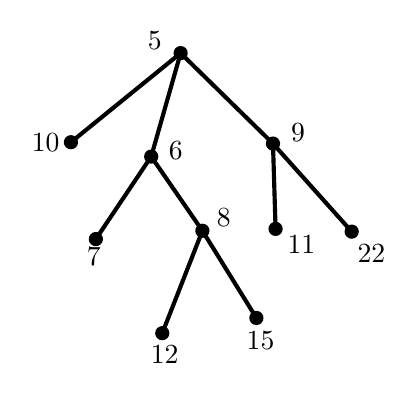
\begin{tikzpicture}[x=0.5pt,y=0.5pt,yscale=-1,xscale=1]
%uncomment if require: \path (0,268); %set diagram left start at 0, and has height of 268

%Flowchart: Connector [id:dp07358279371728427] 
\draw  [fill={rgb, 255:red, 0; green, 0; blue, 0 }  ,fill opacity=1 ] (122.38,22) .. controls (122.38,19.58) and (124.34,17.62) .. (126.75,17.62) .. controls (129.17,17.62) and (131.13,19.58) .. (131.13,22) .. controls (131.13,24.42) and (129.17,26.38) .. (126.75,26.38) .. controls (124.34,26.38) and (122.38,24.42) .. (122.38,22) -- cycle ;
%Flowchart: Connector [id:dp9013708586598245] 
\draw  [fill={rgb, 255:red, 0; green, 0; blue, 0 }  ,fill opacity=1 ] (43.12,86.38) .. controls (43.12,83.96) and (45.08,82) .. (47.5,82) .. controls (49.92,82) and (51.88,83.96) .. (51.88,86.38) .. controls (51.88,88.79) and (49.92,90.75) .. (47.5,90.75) .. controls (45.08,90.75) and (43.12,88.79) .. (43.12,86.38) -- cycle ;
%Flowchart: Connector [id:dp29553697353599095] 
\draw  [fill={rgb, 255:red, 0; green, 0; blue, 0 }  ,fill opacity=1 ] (246,151) .. controls (246,148.58) and (247.96,146.62) .. (250.38,146.62) .. controls (252.79,146.62) and (254.75,148.58) .. (254.75,151) .. controls (254.75,153.42) and (252.79,155.38) .. (250.38,155.38) .. controls (247.96,155.38) and (246,153.42) .. (246,151) -- cycle ;
%Straight Lines [id:da2622599551377074] 
\draw [color={rgb, 255:red, 0; green, 0; blue, 0 }  ,draw opacity=1 ][line width=1.5]    (195.38,149) -- (193.5,87.38) ;
%Straight Lines [id:da633932922371613] 
\draw [color={rgb, 255:red, 0; green, 0; blue, 0 }  ,draw opacity=1 ][line width=1.5]    (47.5,86.38) -- (126.75,22) ;
%Flowchart: Connector [id:dp6006241534205703] 
\draw  [fill={rgb, 255:red, 0; green, 0; blue, 0 }  ,fill opacity=1 ] (101.12,96.75) .. controls (101.12,94.34) and (103.08,92.38) .. (105.5,92.38) .. controls (107.92,92.38) and (109.88,94.34) .. (109.88,96.75) .. controls (109.88,99.17) and (107.92,101.13) .. (105.5,101.13) .. controls (103.08,101.13) and (101.12,99.17) .. (101.12,96.75) -- cycle ;
%Flowchart: Connector [id:dp13162082051454493] 
\draw  [fill={rgb, 255:red, 0; green, 0; blue, 0 }  ,fill opacity=1 ] (189.12,87.38) .. controls (189.12,84.96) and (191.08,83) .. (193.5,83) .. controls (195.92,83) and (197.88,84.96) .. (197.88,87.38) .. controls (197.88,89.79) and (195.92,91.75) .. (193.5,91.75) .. controls (191.08,91.75) and (189.12,89.79) .. (189.12,87.38) -- cycle ;
%Flowchart: Connector [id:dp7155524303373791] 
\draw  [fill={rgb, 255:red, 0; green, 0; blue, 0 }  ,fill opacity=1 ] (61.12,156.38) .. controls (61.12,153.96) and (63.08,152) .. (65.5,152) .. controls (67.92,152) and (69.88,153.96) .. (69.88,156.38) .. controls (69.88,158.79) and (67.92,160.75) .. (65.5,160.75) .. controls (63.08,160.75) and (61.12,158.79) .. (61.12,156.38) -- cycle ;
%Flowchart: Connector [id:dp5160360494307613] 
\draw  [fill={rgb, 255:red, 0; green, 0; blue, 0 }  ,fill opacity=1 ] (138.12,150.38) .. controls (138.12,147.96) and (140.08,146) .. (142.5,146) .. controls (144.92,146) and (146.88,147.96) .. (146.88,150.38) .. controls (146.88,152.79) and (144.92,154.75) .. (142.5,154.75) .. controls (140.08,154.75) and (138.12,152.79) .. (138.12,150.38) -- cycle ;
%Flowchart: Connector [id:dp48925704975832796] 
\draw  [fill={rgb, 255:red, 0; green, 0; blue, 0 }  ,fill opacity=1 ] (109.12,224.38) .. controls (109.12,221.96) and (111.08,220) .. (113.5,220) .. controls (115.92,220) and (117.88,221.96) .. (117.88,224.38) .. controls (117.88,226.79) and (115.92,228.75) .. (113.5,228.75) .. controls (111.08,228.75) and (109.12,226.79) .. (109.12,224.38) -- cycle ;
%Flowchart: Connector [id:dp46343000023437764] 
\draw  [fill={rgb, 255:red, 0; green, 0; blue, 0 }  ,fill opacity=1 ] (177.12,213.38) .. controls (177.12,210.96) and (179.08,209) .. (181.5,209) .. controls (183.92,209) and (185.88,210.96) .. (185.88,213.38) .. controls (185.88,215.79) and (183.92,217.75) .. (181.5,217.75) .. controls (179.08,217.75) and (177.12,215.79) .. (177.12,213.38) -- cycle ;
%Straight Lines [id:da8627932820811317] 
\draw [color={rgb, 255:red, 0; green, 0; blue, 0 }  ,draw opacity=1 ][line width=1.5]    (105.5,96.75) -- (126.75,22) ;
%Straight Lines [id:da5409521442924461] 
\draw [color={rgb, 255:red, 0; green, 0; blue, 0 }  ,draw opacity=1 ][line width=1.5]    (193.5,87.38) -- (126.75,22) ;
%Straight Lines [id:da6747902580631686] 
\draw [color={rgb, 255:red, 0; green, 0; blue, 0 }  ,draw opacity=1 ][line width=1.5]    (65.5,156.38) -- (105.5,96.75) ;
%Straight Lines [id:da9660976210409085] 
\draw [color={rgb, 255:red, 0; green, 0; blue, 0 }  ,draw opacity=1 ][line width=1.5]    (142.5,150.38) -- (105.5,96.75) ;
%Straight Lines [id:da7815420677213977] 
\draw [color={rgb, 255:red, 0; green, 0; blue, 0 }  ,draw opacity=1 ][line width=1.5]    (113.5,224.38) -- (142.5,150.38) ;
%Straight Lines [id:da6594188595232979] 
\draw [color={rgb, 255:red, 0; green, 0; blue, 0 }  ,draw opacity=1 ][line width=1.5]    (181.5,213.38) -- (142.5,150.38) ;
%Flowchart: Connector [id:dp9035939512481367] 
\draw  [fill={rgb, 255:red, 0; green, 0; blue, 0 }  ,fill opacity=1 ] (191,149) .. controls (191,146.58) and (192.96,144.62) .. (195.38,144.62) .. controls (197.79,144.62) and (199.75,146.58) .. (199.75,149) .. controls (199.75,151.42) and (197.79,153.38) .. (195.38,153.38) .. controls (192.96,153.38) and (191,151.42) .. (191,149) -- cycle ;
%Straight Lines [id:da9909770061710292] 
\draw [color={rgb, 255:red, 0; green, 0; blue, 0 }  ,draw opacity=1 ][line width=1.5]    (250.38,151) -- (193.5,87.38) ;

% Text Node
\draw (116,84) node [anchor=north west][inner sep=0.75pt]   [align=left] {$\displaystyle 6$};
% Text Node
\draw (172.24,221.06) node [anchor=north west][inner sep=0.75pt]   [align=left] {$\displaystyle 15$};
% Text Node
\draw (56.75,160) node [anchor=north west][inner sep=0.75pt]   [align=left] {$\displaystyle 7$};
% Text Node
\draw (204.38,70.38) node [anchor=north west][inner sep=0.75pt]   [align=left] {$\displaystyle 9$};
% Text Node
\draw (252.38,158.38) node [anchor=north west][inner sep=0.75pt]   [align=left] {$\displaystyle 22$};
% Text Node
\draw (201.75,152) node [anchor=north west][inner sep=0.75pt]   [align=left] {$\displaystyle 11$};
% Text Node
\draw (150.75,132.35) node [anchor=north west][inner sep=0.75pt]   [align=left] {$\displaystyle 8$};
% Text Node
\draw (102.97,230.91) node [anchor=north west][inner sep=0.75pt]   [align=left] {$\displaystyle 12$};
% Text Node
\draw (16.97,77.91) node [anchor=north west][inner sep=0.75pt]   [align=left] {$\displaystyle 10$};
% Text Node
\draw (100.75,4.35) node [anchor=north west][inner sep=0.75pt]   [align=left] {$\displaystyle 5$};


\end{tikzpicture}

